\chapter{Urinveier}%urinveiene
		\section{Gullkornene:}
			\begin{itemize}
				\item Vanligere med urinveisinfeksjon i høyere alder.\\
				\item En vanlig årsak til delir(se side \pageref{delir}).\\
				\item Bakterier i urinen til gamle damer behøver ikke være farlig.\\
				\item Lukt og farge kan lure oss.\\
			\end{itemize}
		\section{Anatomi}
					\begin{figure}[ht]
                      \centering
                      	\frame{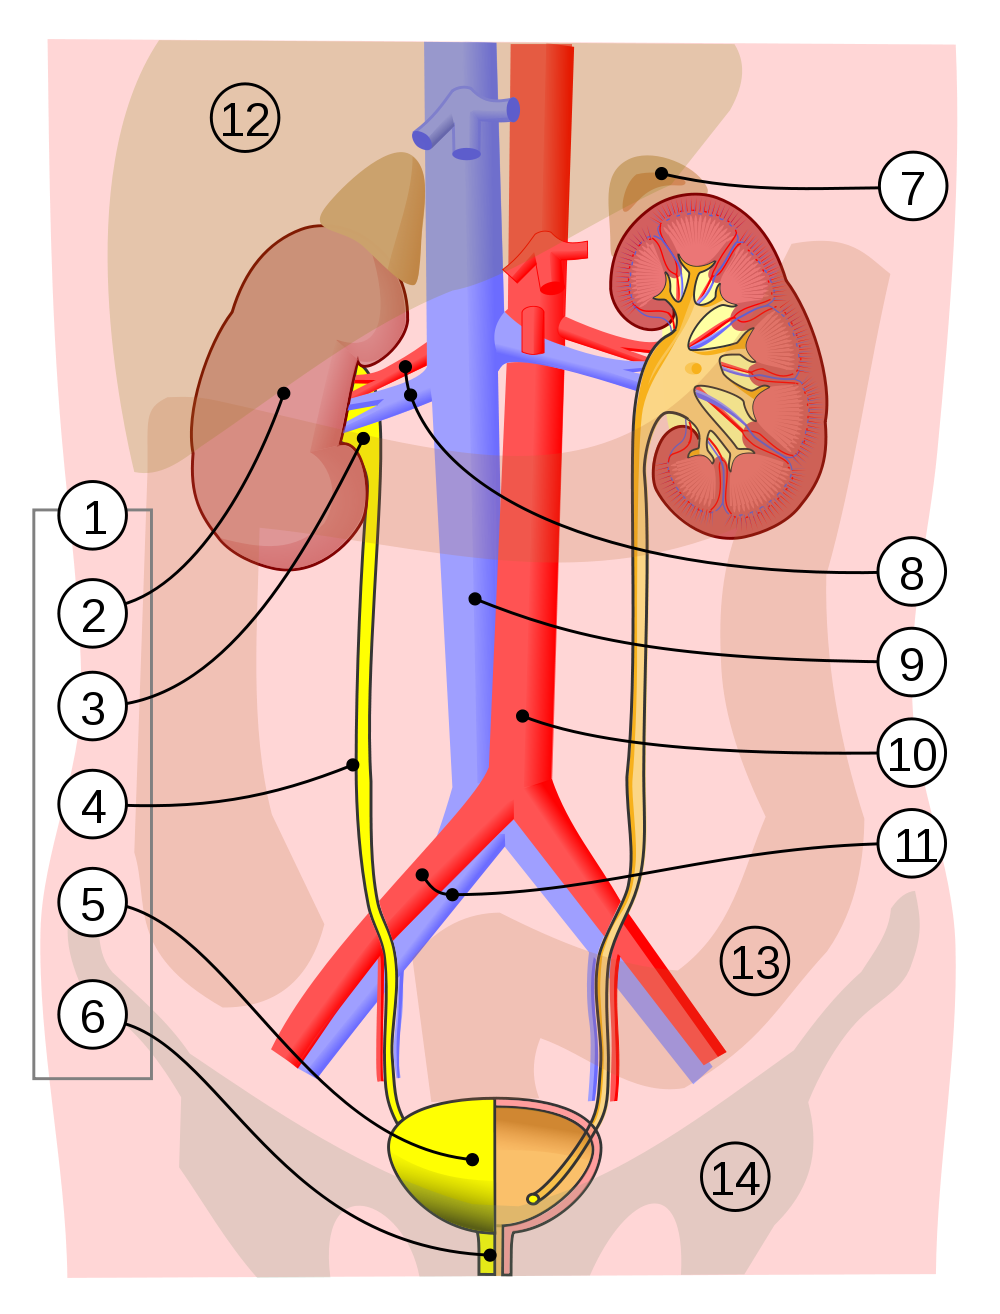
\includegraphics[width=5in]{./kap/bilder/urinveier.png}}%!!! må byttes ut, copyright Greys anatomy
                      \caption{\emph{1.} Urinveiene ,\emph{2.} Nyre, \emph{3.} Nyrebekkenet, \emph{4.} Urether, \emph{5.} Blæra, \emph{6.} Urethra, \emph{7.} Binyre, \emph{8.} Nyrearterie og -vene, \emph{9.} Vena cava inferior, \emph{10.} Bukaorta, \emph{11.} Arteria og Vena Iliaca, \emph{12.} Lever, \emph{13.} Tykktarmen, \emph{14.} Bekkenet}
                    \end{figure}
			\paragraph{Feilkonstruksjon?\\}
				Kvinner har et kort urinrør som gjør det svært lett å få urinveisinfeksjoner. At eldre damer har bakterier i urinen uten symptomer er forholdsvis vanlig og ikke farlig\cite{uti-old}
			\paragraph{Den svake strålen\\}
				Menn har også hyppigere infeksjoner med alderen. Det er ofte prostaten, plager etter operasjon og kateterbruk som gjør dette. 
		\section{Fysiologi}
			Bakteriene vandrer nedenfra og opp. Urin er steril hos friske. Eldre med bakterier uten symptomer trenger vanligvis ikke behandling. 
		\section{Patologi}
			\paragraph{Flere nivåer\\}
				Bakteriene irriterer lokalt og skaper smerter når man er på do. Noen får generell slapphet av den pågående reaksjonen. Hvis bakteriene kommer opp til nyrene kalles det pyelonefritt, eller nyrebekkenbetennelse. Kommer de enda høyere kalles det urosepsis og er kjennetegnet av at bakteriene sprer seg i hele kroppen via blodet. 
		\section{Klinikk}
			\subsection{UVI}
				Veldig vanlig og trenger ikke behandling dersom fravær av symptomer. Pasienten bør følges tett dersom bakterier påvises, for deretter å kunne slippe opp litt. Man i disse pasientene huske på at urinveiene an være årsak ved sykdom. Ta urinprøver regelmessig, men det behøver ikke føre til behandling.
		\section{Pasienteksempler}
			\subsection{Pasient 7}
				Hva skjer Jakob(75)? Han har vært enkemann i 4 år, våken og klar men har hjelp av hjemmetjenesten, fordi han må katetrisere seg flere ganger daglig på grunn av protataen. Ved dagens besøk har forberedt et bål midt på stuegulvet og hjemmetjenesten møtes av Jakob som har på solbrille underbukse og ikke mye annet. Han forteller at det må en avbrenning til å fjerne den lille mannen med motorsykkel som raser rundt oppunder taket. 
				\begin{enumerate}
					\item Hva gjør du?
					\item Kan denne pasienten behandles hjemme?
					\item Hva er prognosen?
					\item Hvilken test bør gjennomføres så snart som mulig?
				\end{enumerate}
			\subsection{Pasient 8}
				Laila er 84 og bor med sin mann. Hjemmetjenesten kontaktes av fastlegen som har hatt mannen på besøk i dag. Han forteller at Laila ikke klarer seg selv lengre. Hun er gradvis blitt dårligere. Etter vurderingsbesøket er det klart at hun må på sykehus: Hun er helt psykotisk og hallusinerende.\par
				Etter 4 dager er hun utskrevet til hjemmet og det er bedt om et vurderingsbesøk. Hun virker nå mye slappere, ligger rett ut. Klarer ikke bøye armer og ben. Sløv og trett men hallusinerer ikke.
				\begin{enumerate}
						\item Hvilken mye brukt medisin i behandlingen av psykoser er årsaken til dette?
						\item Må du ringe legevakt eller ambulanse eller kan du avvente videre?
						\item Hva forventer du står i brevet fra sykehuset?
						\item Hva er forskjellen på delir og psykose? 
						\item Hva forteller du til hennes pårørende som lurer på hva som skjer med tante Laila?
					\end{enumerate}